\section{Results}
\label{sec:results}

\subsection{Extraction Statistics}
\label{sec:results:extraction}

From 150 Wikipedia articles, our probe-free method extracts 7{,}405 multi-token segment instances (6{,}494 unique) through greedy segmentation.
The mean combined score is 0.532 (median 0.591), with scores spanning the full $[0, 1]$ range.
\Figref{fig:score_dist} shows the distribution of combined scores and its component signals.
As a reference, spaCy NER detects 3{,}185 named entities in the same corpus, and 76.1\% of our extracted items overlap with at least one NER entity.

\begin{figure}[t]
    \centering
    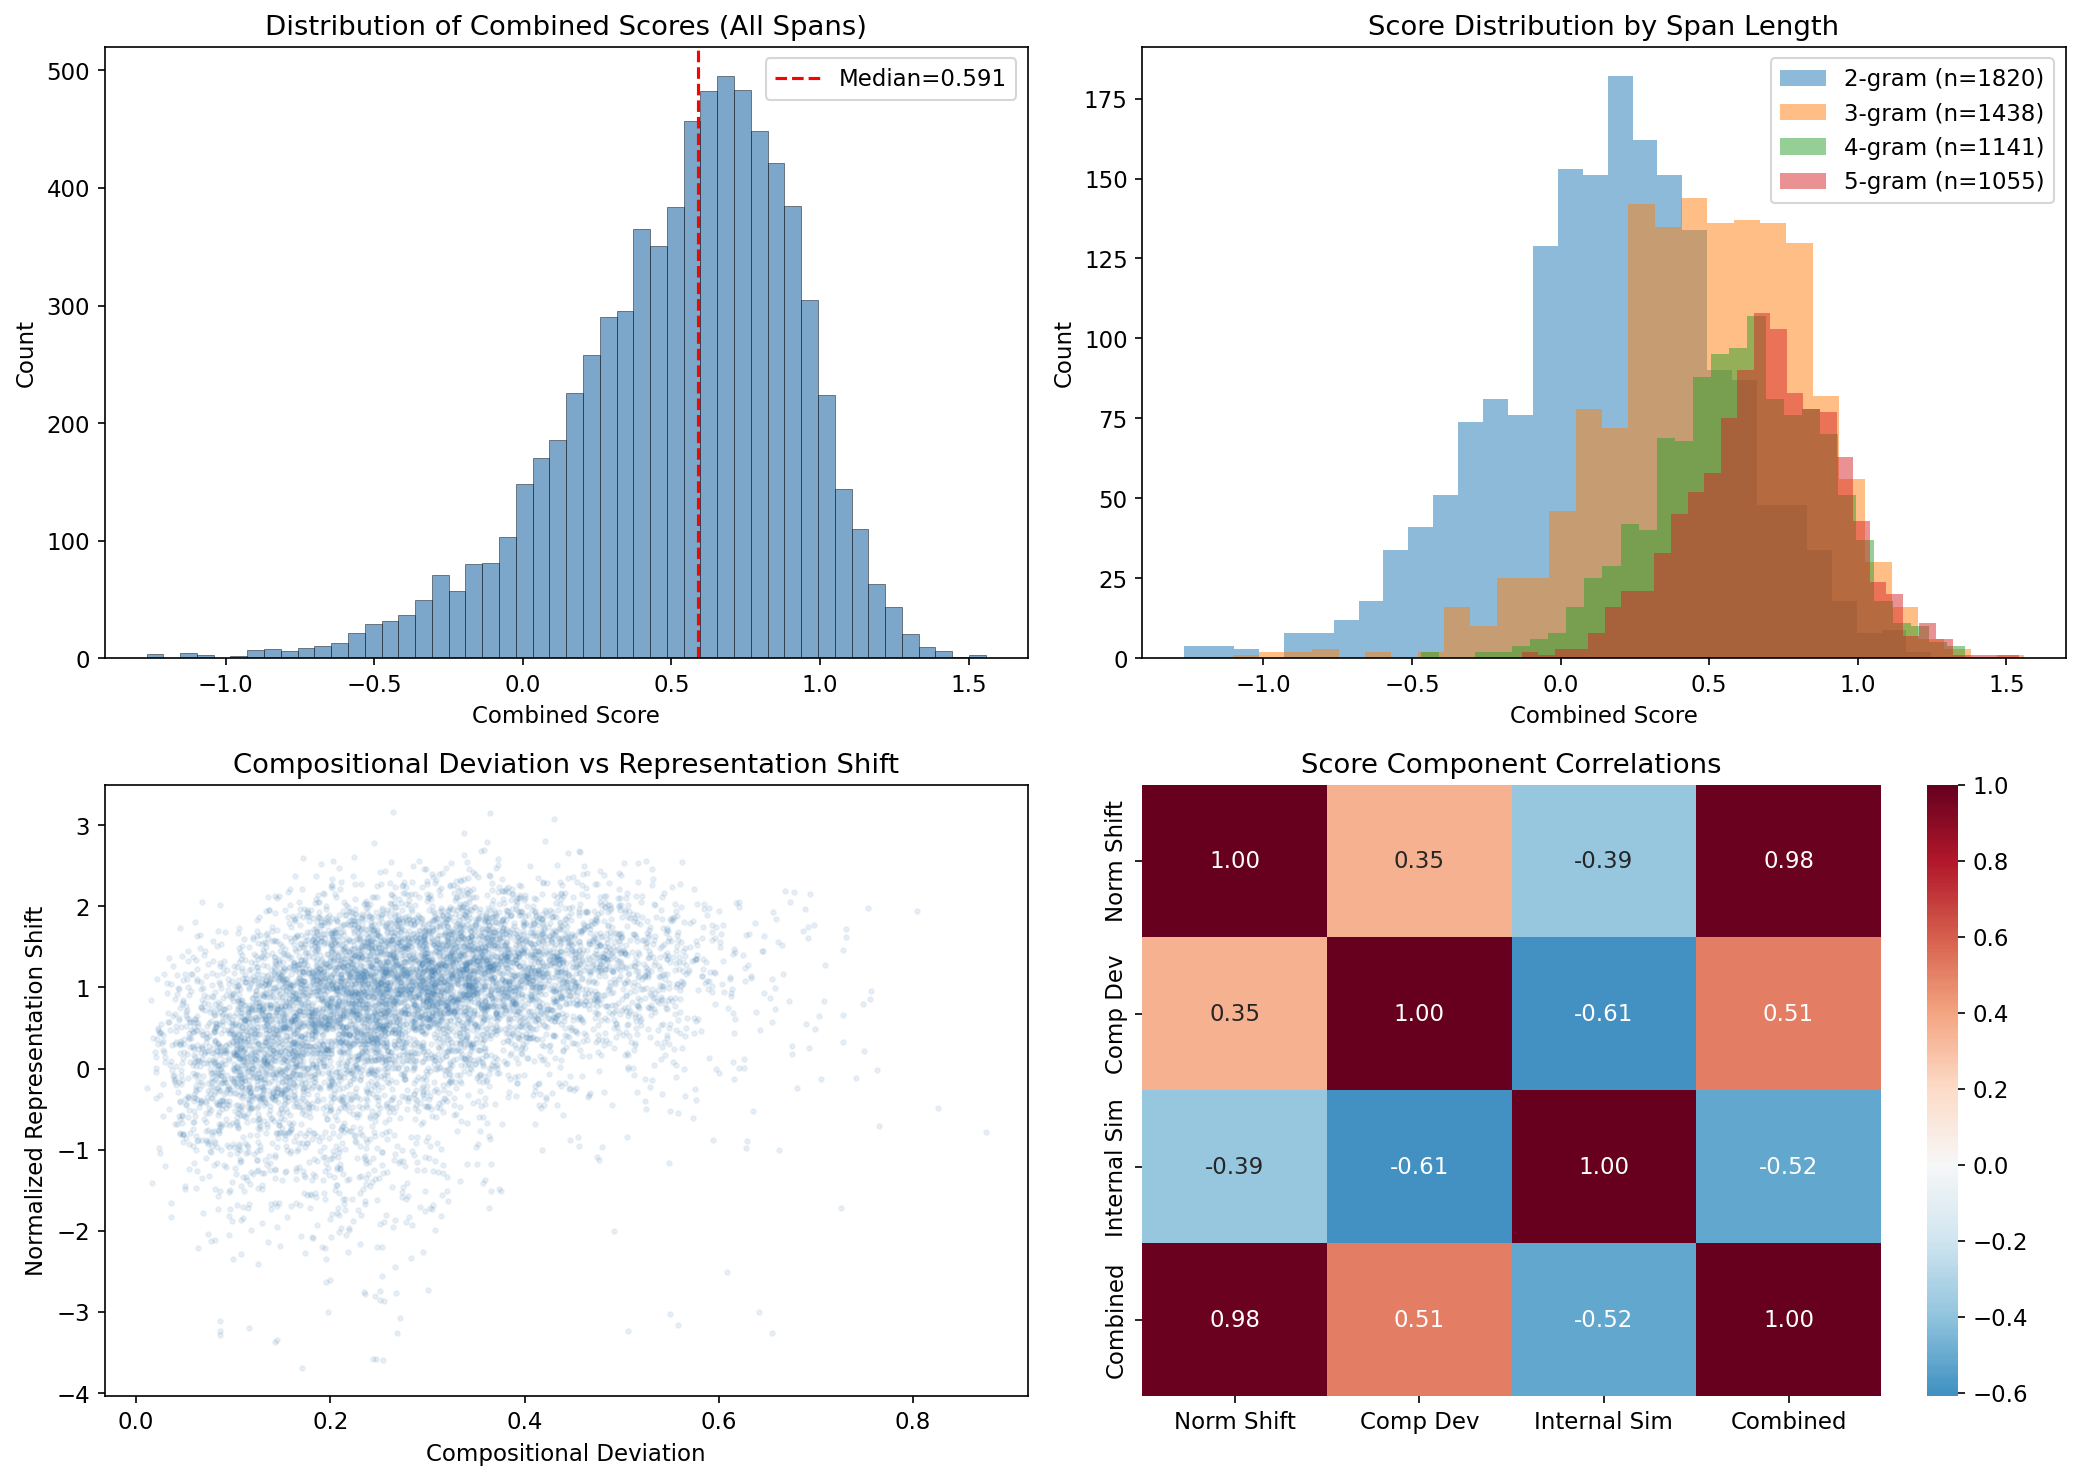
\includegraphics[width=0.95\linewidth]{figures/score_distributions.png}
    \caption{Distribution of combined scores and component signals. \figleft Combined score distribution across all extracted items. \figright Relationship between compositional deviation and representation shift, the two primary components of the combined score.}
    \label{fig:score_dist}
\end{figure}

\subsection{Compositionality Analysis}
\label{sec:results:compositionality}

\para{Category distribution.}
\Tabref{tab:categories} shows the classification results for 500 stratified items.
Fragments---meaningless token spans such as partial words split across BPE boundaries (\eg ``arus which forbids'')---account for 48\% of items, indicating that the probe-free method has higher noise than probe-based erasure.
Among the 260 meaningful items, named entities are the largest category (38.1\%), followed by compositional phrases (28.5\%), technical terms (15.4\%), fixed expressions (11.5\%), compound words (5.8\%), and idioms (0.8\%).

\begin{table}[t]
    \centering
    \caption{Classification of 500 stratified implicit vocabulary items by GPT-4.1. We report counts, percentages, mean compositionality scores (0 = fully non-compositional, 1 = fully compositional), and mean erasure-like scores. Best compositionality discrimination in \textbf{bold}.}
    \label{tab:categories}
    \begin{tabular}{@{}lcccc@{}}
        \toprule
        \textbf{Category} & \textbf{Count} & \textbf{\%} & \textbf{Comp.} & \textbf{Score} \\
        \midrule
        Fragment & 240 & 48.0 & 0.327 & 0.531 \\
        Named entity & 99 & 19.8 & \textbf{0.379} & 0.623 \\
        Compositional phrase & 74 & 14.8 & 1.000 & 0.586 \\
        Technical term & 40 & 8.0 & 0.740 & \textbf{0.733} \\
        Fixed expression & 30 & 6.0 & 0.730 & 0.480 \\
        Compound word & 15 & 3.0 & 0.687 & 0.641 \\
        Idiom & 2 & 0.4 & 0.300 & 0.339 \\
        \bottomrule
    \end{tabular}
\end{table}

\para{Score--compositionality correlation.}
Among the 260 meaningful items (excluding fragments), we find a significant negative correlation between the combined score and compositionality (Spearman $\rho = -0.182$, $p = 0.003$).
\Figref{fig:comp_vs_score} visualizes this relationship, showing that higher-scoring items cluster toward lower compositionality values.

\begin{figure}[t]
    \centering
    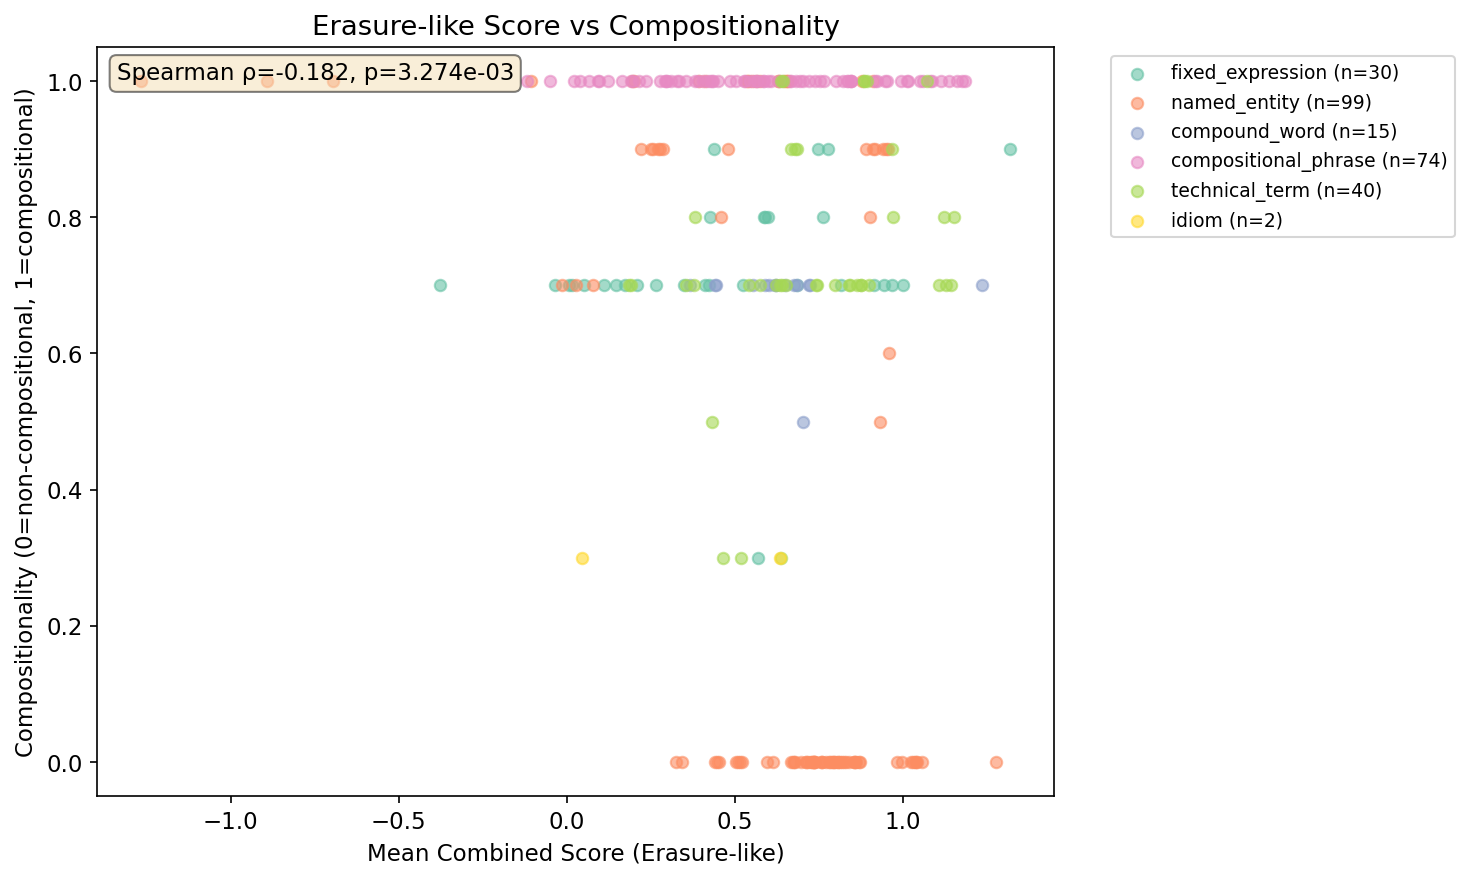
\includegraphics[width=0.95\linewidth]{figures/compositionality_vs_score.png}
    \caption{Compositionality rating vs.\ erasure-like score for 260 meaningful implicit vocabulary items, colored by category. The negative correlation (Spearman $\rho = -0.182$, $p = 0.003$) confirms that items the model treats as unified units tend to be less compositional.}
    \label{fig:comp_vs_score}
\end{figure}

\para{High vs.\ low score comparison.}
Splitting meaningful items at the median combined score, high-scoring items have a mean compositionality of 0.557 compared to 0.781 for low-scoring items (Mann-Whitney $U = 6{,}117.5$, $p < 0.0001$, Cohen's $d = -0.60$).
This medium effect size confirms that the model's internal representation shifts preferentially target non-compositional sequences.

\subsection{Statistical Tests}
\label{sec:results:stats}

\Tabref{tab:stats} summarizes our statistical tests.
The core finding---that higher erasure-like scores predict lower compositionality---is robust across multiple tests.
The category distribution is highly non-uniform ($\chi^2 = 155.5$, $p < 10^{-31}$), dominated by named entities.
Notably, the overall compositionality of extracted items does \emph{not} differ significantly from low-score baseline items ($U = 50{,}637$, $p = 0.781$), because the extraction process captures both compositional and non-compositional items; the discrimination occurs \emph{within} the score distribution.

\begin{table}[t]
    \centering
    \caption{Statistical tests. All tests use $\alpha = 0.05$.}
    \label{tab:stats}
    \resizebox{\textwidth}{!}{%
    \begin{tabular}{@{}llll@{}}
        \toprule
        \textbf{Test} & \textbf{Statistic} & \textbf{$p$-value} & \textbf{Effect size} \\
        \midrule
        Score--compositionality correlation & Spearman $\rho = -0.182$ & 0.003 & Small--medium \\
        High vs.\ low score compositionality & $U = 6{,}117.5$ & $< 0.0001$ & $d = -0.60$ (medium) \\
        Non-comp.\ vs.\ comp.\ categories & $U = 999.0$ & $< 10^{-27}$ & $d = -1.72$ (large) \\
        Vocabulary vs.\ baseline compositionality & $U = 50{,}637.0$ & 0.781 & n.s. \\
        Category distribution vs.\ uniform & $\chi^2 = 155.5$ & $< 10^{-31}$ & --- \\
        \bottomrule
    \end{tabular}
    }
\end{table}

\subsection{Category-Level Analysis}
\label{sec:results:category}

\Figref{fig:category} shows compositionality and score distributions by category.
Named entities have the lowest mean compositionality (0.379) among meaningful categories, consistent with their non-compositional nature: ``CompuServe'' cannot be derived from ``Compu'' and ``Serve.''
Technical terms show the highest mean erasure-like score (0.733), suggesting particularly strong representation merging for domain-specific terminology.
Fixed expressions and compound words occupy a middle ground (compositionality 0.687--0.730), reflecting their partially compositional nature.

\begin{figure}[t]
    \centering
    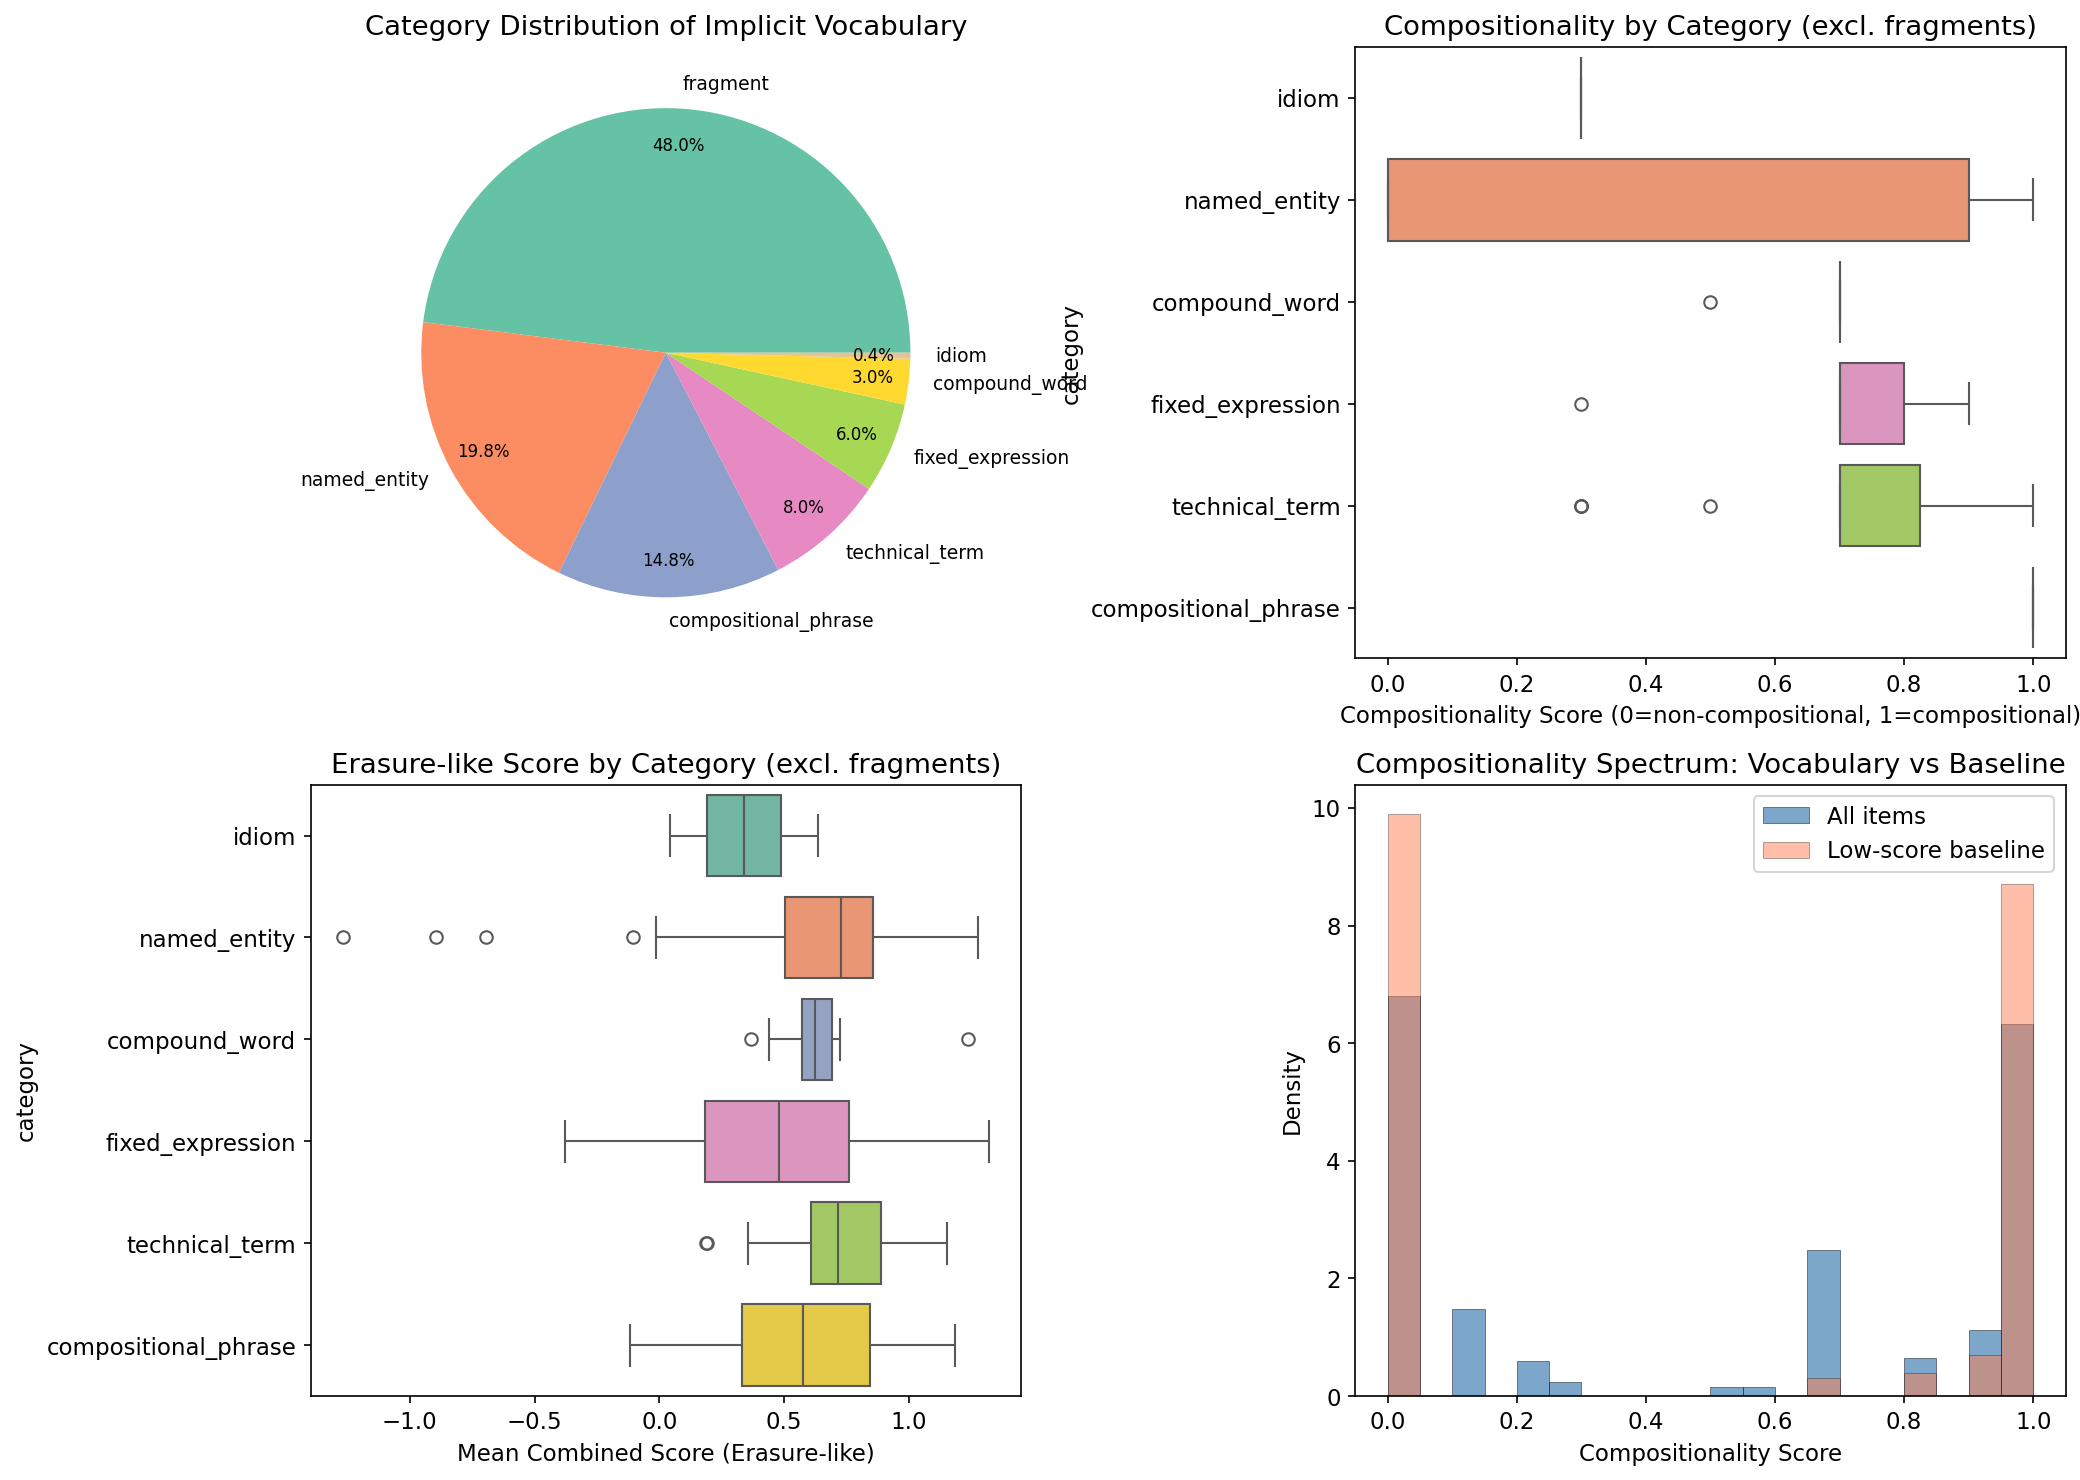
\includegraphics[width=0.95\linewidth]{figures/category_analysis.png}
    \caption{Category-level analysis of implicit vocabulary items. The figure shows the distribution of categories, compositionality scores by category, erasure-like scores by category, and the compositionality spectrum comparing vocabulary items to the low-score baseline. Named entities and idioms cluster at low compositionality, while compositional phrases are at 1.0 by definition.}
    \label{fig:category}
\end{figure}

\subsection{NER Overlap Analysis}
\label{sec:results:ner}

\Figref{fig:ner} shows the overlap between our extracted implicit vocabulary and spaCy NER entities.
Of the 6{,}494 unique extracted items, 76.1\% overlap with at least one NER entity, confirming that named entities are heavily represented in the implicit vocabulary.
NER-matching items show slightly higher erasure-like scores than non-NER items, consistent with our finding that the model treats named entities with strong merging behavior.

\begin{figure}[t]
    \centering
    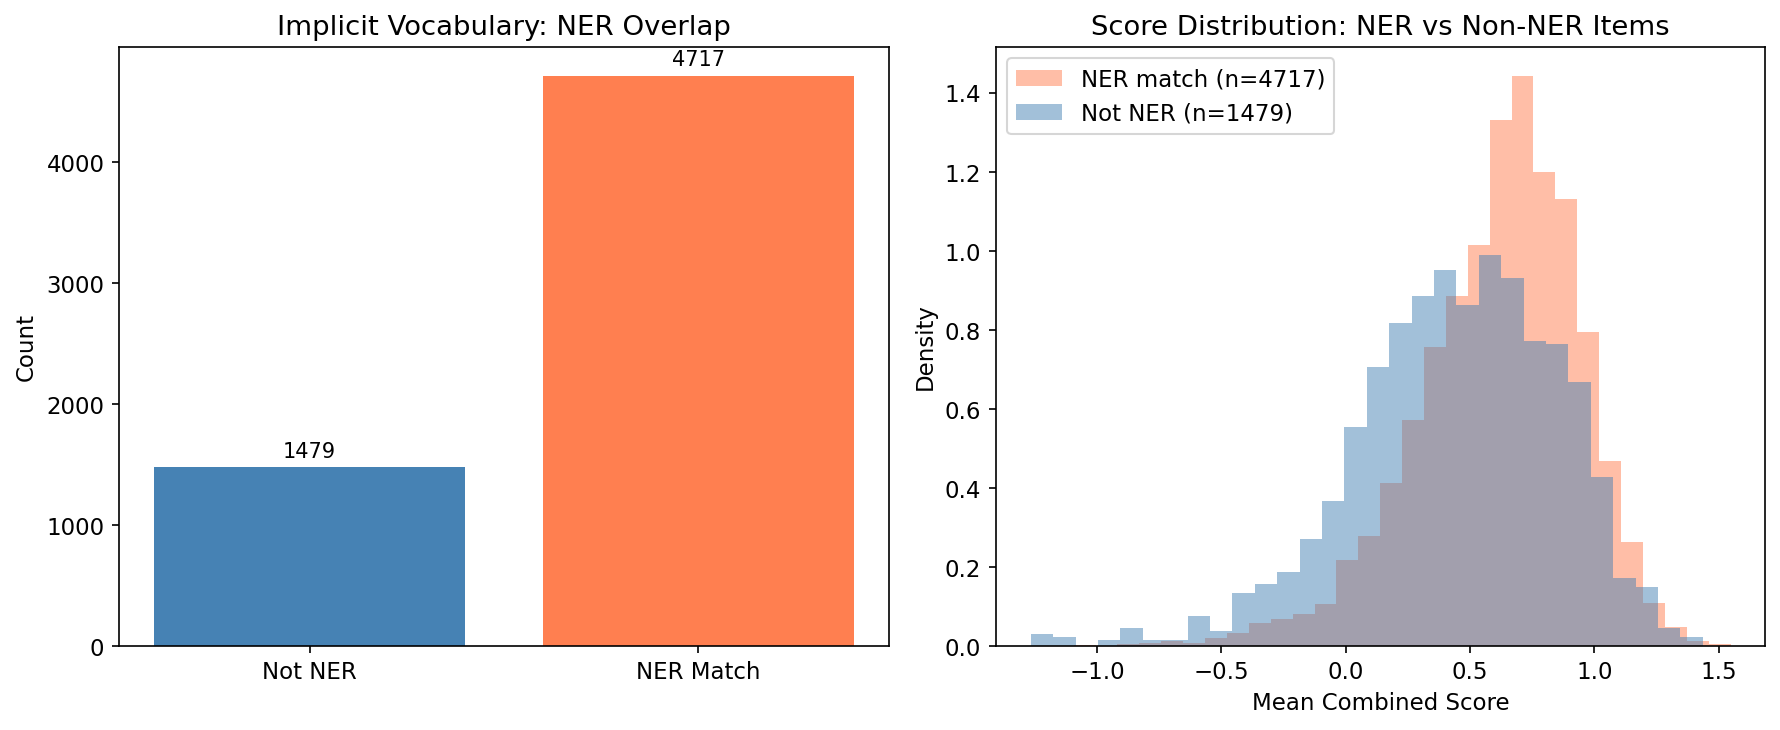
\includegraphics[width=0.95\linewidth]{figures/ner_analysis.png}
    \caption{NER overlap analysis. 76.1\% of extracted implicit vocabulary items overlap with spaCy NER entities. NER-matching items show a rightward shift in the score distribution, indicating slightly higher erasure-like scores.}
    \label{fig:ner}
\end{figure}

\subsection{Vocabulary Size}
\label{sec:results:vocabsize}

\Figref{fig:vocabsize} shows how the size of the implicit vocabulary changes as a function of the combined score threshold.
At no threshold, all 6{,}494 unique items are included.
Raising the threshold progressively filters out lower-scoring items, yielding a more selective vocabulary dominated by named entities and technical terms.
The distribution of span lengths peaks at 2--3 tokens, with longer spans (5--6 tokens) being rarer.

\begin{figure}[t]
    \centering
    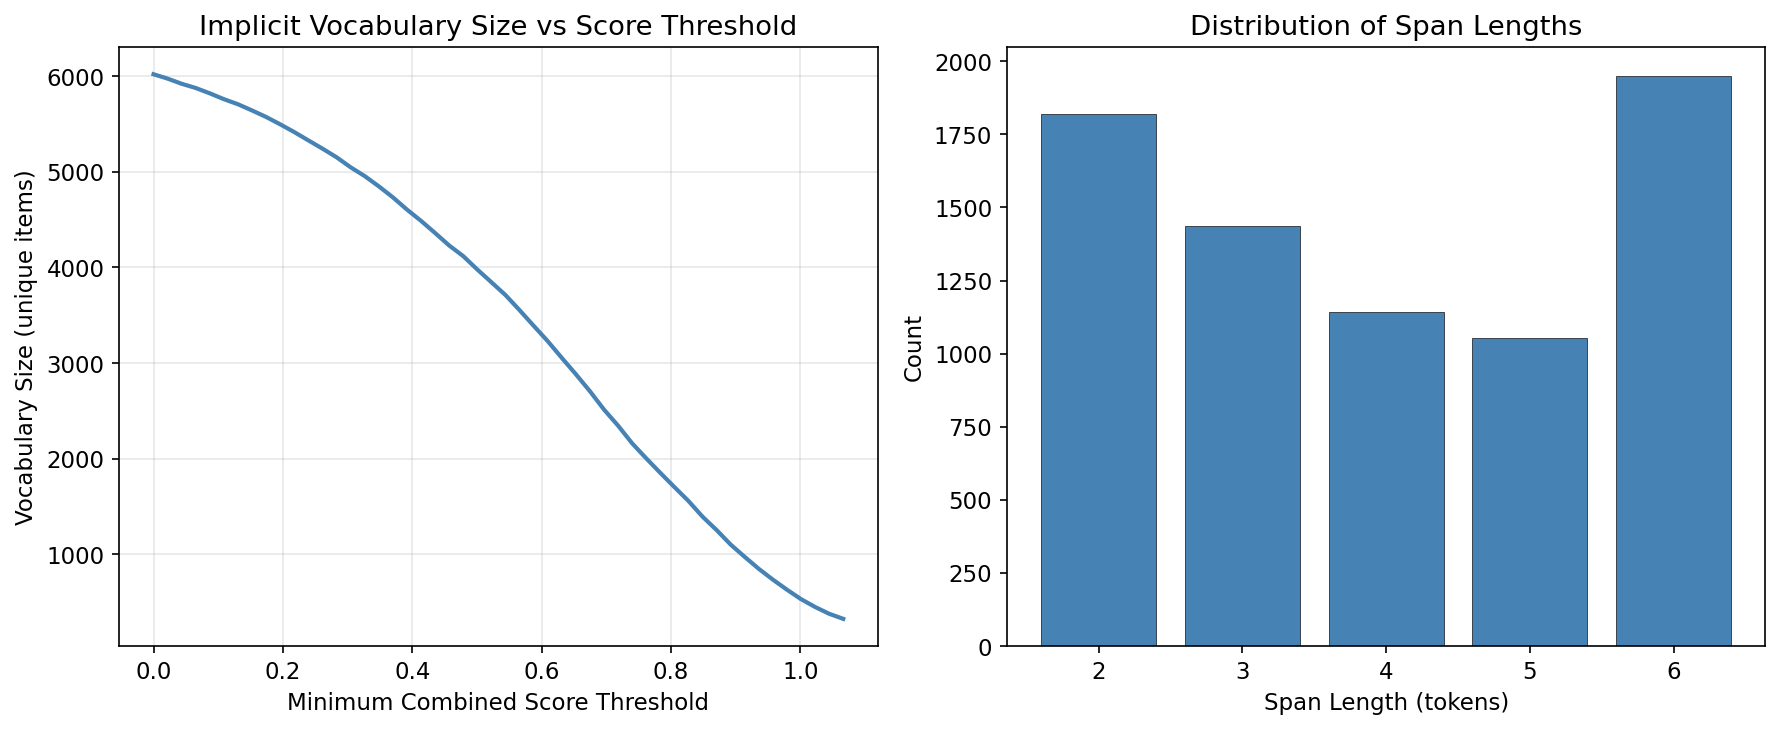
\includegraphics[width=0.95\linewidth]{figures/vocabulary_size.png}
    \caption{Vocabulary size as a function of combined score threshold (left) and distribution of span lengths among extracted items (right). Most implicit vocabulary items consist of 2--3 tokens.}
    \label{fig:vocabsize}
\end{figure}
